\chapter{Progettazione concettuale}
    \section{Diagramma ER}
        Dall'analisi dei requisiti costruiamo il diagramma ER.\\
        In particolare, il modello concettuale basato sull'analisi dei requisiti permetterà di creare una base di dati efficace per la gestione del personale e delle attività svolte nell'azienda.\\
        Il modello dovrà tenere in considerazione le due tipologie di dipendenti e le relative informazioni tracciate nella base di dati, i laboratori, i progetti, i fondi e gli acquisti effettuati tramite i fondi.\\\\
        \begin{figure}[htbp!]
            \centering
                \vspace{4\baselineskip}
                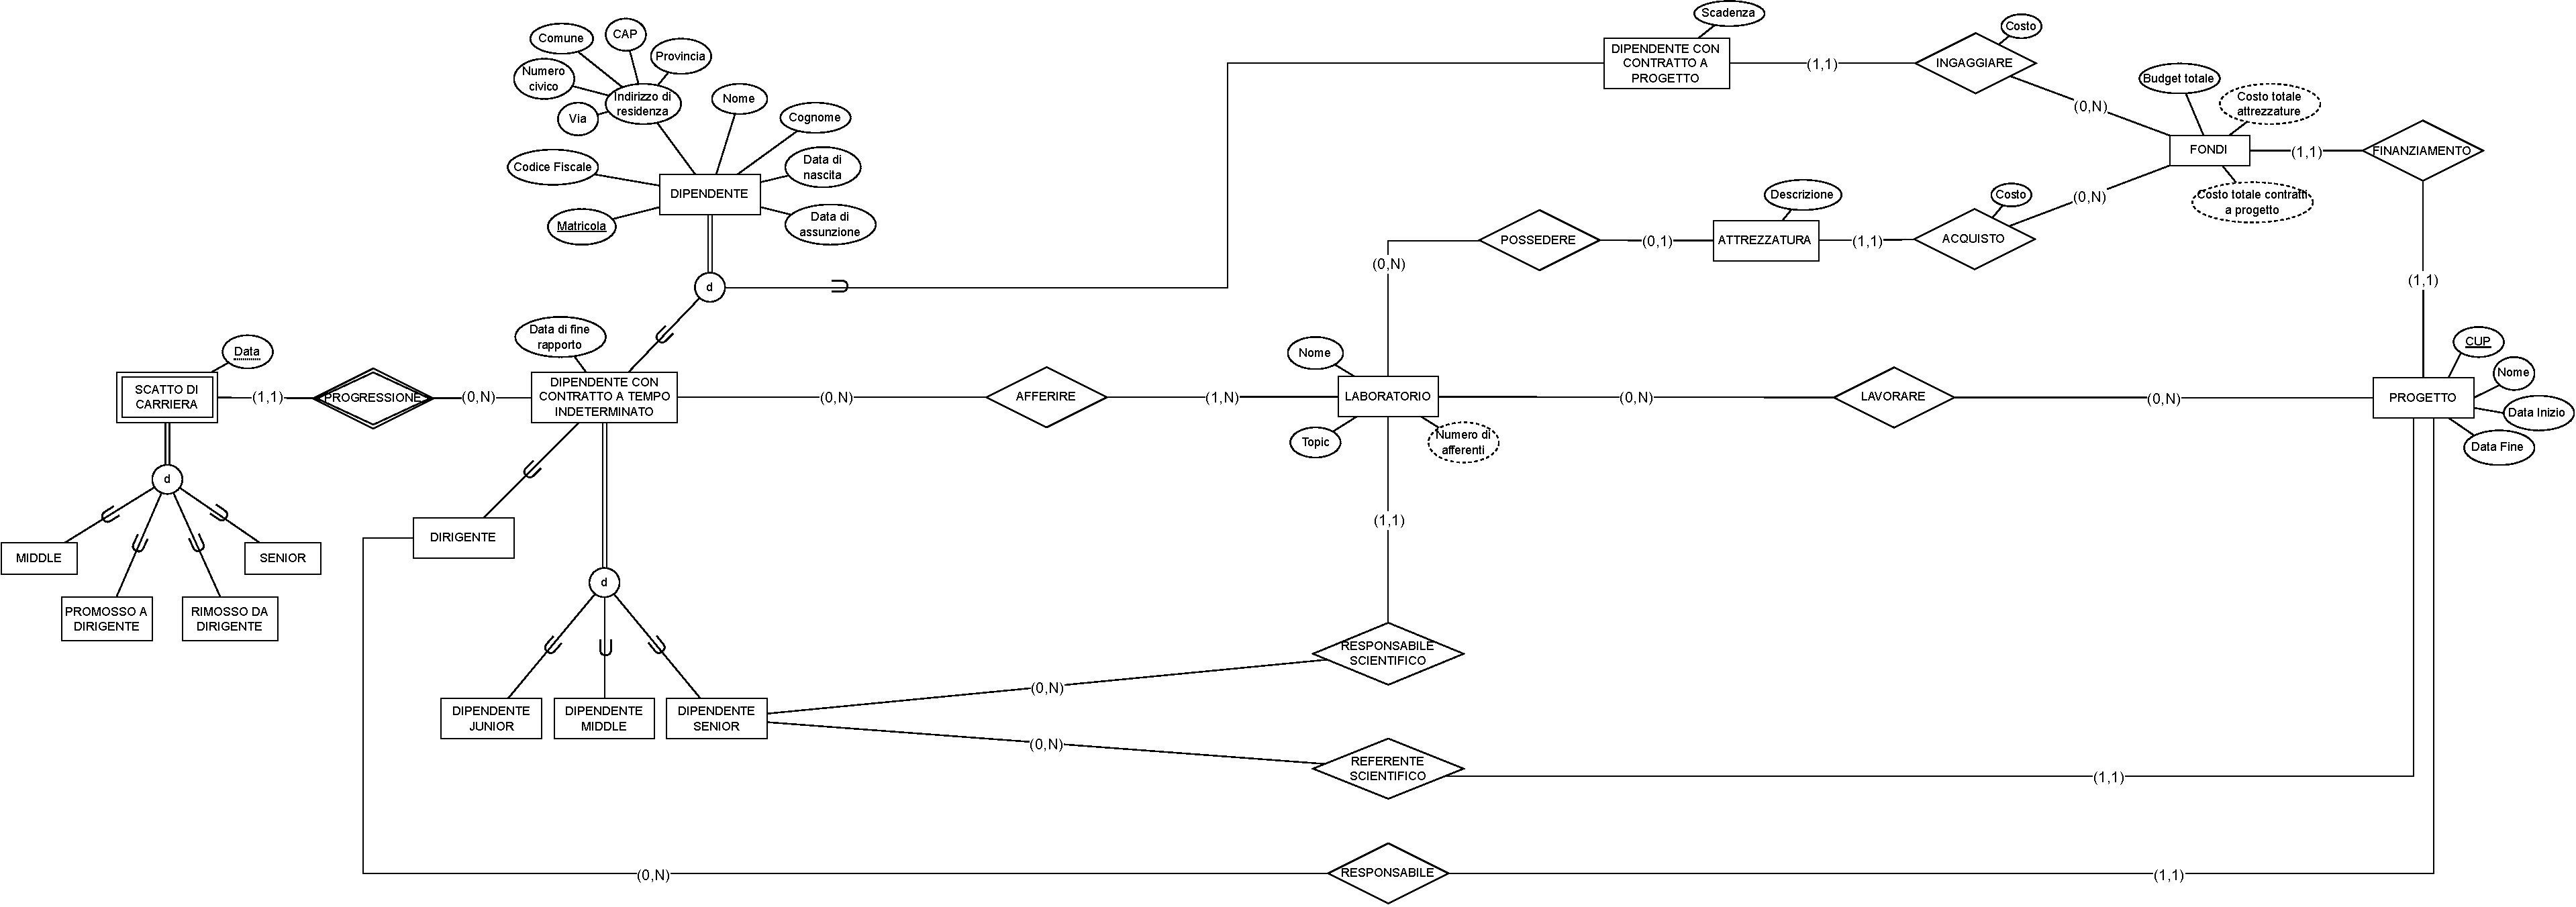
\includegraphics[width=\linewidth]{Diagrammi/Diagramma ER non ristrutturato.pdf}
            \caption{Diagramma ER non ristrutturato}
            \label{fig:Diagramma ER non ristrutturato}
        \end{figure}